\chapter{Introduction}
Machine learning algorithms are nowadays important topic when we are challenging learning from many more data than before. Deep learning is promising technique to enhance machine learning performance on many tasks. Innovation over other machine learning algorithms is that we are able to express objects as a set of gradually more complex features. This natural expression makes it possible to get much more knowledge about data. As a front page article 2012 New York Times wrote \textit{"advances in an artificial intelligence technology that can recognize patterns offer the possibility of machines that perform human activities like seeing, listening and thinking"}. This is very far fetch conclusion about this topic, nevertheless we are already doing impressive things by using this technique. Deep learning is using deep neural networks as a instrument to encode and learn object features.

Idea about artificial neural networks is much deeper than just machine learning algorithm. Inspiration to this model is most complex part of human body - brain. In computational neuroscience is this artificial model used to create link to his biological sibling in order to understand how this intelligent system might work. Also neural networks as a computational system could be interesting alternative to our standard sequential model.

Today in fact artificial neural network is a complex learning algorithm but yet is still very incomplete. Many research groups are coming up with improvements. By combining these ideas we are able to find neural networks as a state-of-the-art algorithm in many machine learning tasks. But especially on non crafted tasks, performance of this algorithm is still incomparable to human performance. Here are some interesting uses of neural networks. The NASA Intelligent Flight Control System which enhance flight control system enabling pilot to maintain control and safely land an aircraft that has suffered a failure. Stanford computer scientists created system that can learn helicopter's to perform stunts only by watching. The DARPA SyNAPSE program is trying to build a computer which architecture is similar to brain. Such computer would be used to build robot's with intelligence of mice or cat. Ilya Sutskever created network which by reading Wikipedia was able to understand some syntax and semantics of human languages.

Computer vision is one of the main domain for neural networks and historically first practical successes in deep learning for this system were proven in digit recognition[LeNet]. By consistently taking prizes from vision competitions they are nowadays considered as a state of the art algorithm for this subject [ILSVRC-2012]. By little tweaking to classical feed forward network we are able to create  model which can learn powerful features from input by continuously applying convolution. This models are called convolutional neural networks. Interestingly enough is this model inspired by primate visual cortex thus mimics most powerful vision system known. Hubel and Wiesel experiments showed that when they projected patterns in front of a cat at different angles different neurons responded. Same happened for dark and light patterns. These neurons are referred as simple cells and their primary function is edge detection. Other neurons termed complex cells responded to those patters regardless of their spatial variance. These types of cells are creating hierarchy where complex cells are receiving input from simple cells and their receptive field is then summation of simple cells receptive fields. Convolutional neural networks are using multiple stages of simple/complex cells combination to gradually learn object feature detectors.

My practical part of thesis will describe experimenting with various techniques and parameters on Alex Krizhevsky's framework which is fast C++/CUDA implementation of convolutional neural network. I will be working with natural image dataset Caltech101. Model learning can be sometimes challenging. It needs to set a lot of parameters which require lot of knowledge about algorithm as well as a great deal of experimenting. Another flaw is that they are also very computationally expensive which is one of a main reason they were unpopular for so long. Alex's framework enables me to set a lot of parameters easily and require only minor changes to make him work with a new dataset. For efficient learning i will use GeForce GTX 680 graphic card. 

Chapters are focused on theoretical description of neural network model. Beginning by logistic regression where you may find some basics about machine learning and classification. Leading through non-linear hypothesis which is describing why we need complicated models like neural networks to represent data features. At the end of this theoretical section is described transformation of classical neural network to convolutional neural network. In chapter you may find detailed description of experiments, reached results as well as tool I used. 

\chapter{Basic principles of classification}
\section{Logistic regression}
Logistic Regression is a statistical model which we can see as an simple object classification algorithm. Output of this model is saying what is a probability that our input belongs to some class. In basic form model can distinguish between two classes but can be generalize to any number of classes. Logistic regression can be seen as a basic building block for deep neural networks. Base of this algorithm is sigmoid function hypothesis. This function takes as a parameters model weights \(\theta\) and input \(x\). We call this function a hypothesis. I will use vectorize notation which is commonly used in neural networks.

\begin{equation}
\label{hypothesis}
h_\theta (x) = \frac{1}{1+e^{-(\theta x)}}
\end{equation}

This hypothesis is telling us what is model thinking in his current configuration. That mean what is an output of the model with his current setting of weights. If we plot this function we will see that \(0 \leq h_\theta \leq 1\). This property makes this algorithm suitable for classification because if we add some threshold we can assign output of a hypothesis to one of two classes. This unit is then called binary decision unit.

For purpose of illustration we define our training data to have two features \(x1\) and \(x2\) which belongs to one of two classes. This non-linear boundary can look like this and it is set by the multiplication of model parameters with his input. Green triangles are data belonging to first class, yellow ones are data belonging to second class. In our example with threshold 0.5 function predicts 1 if \( x1^2 + x2^2-1 \geq 0 \) otherwise 0.

\begin{table}[ht]
\begin{tabular}{*{2}{m{0.4\textwidth}}}
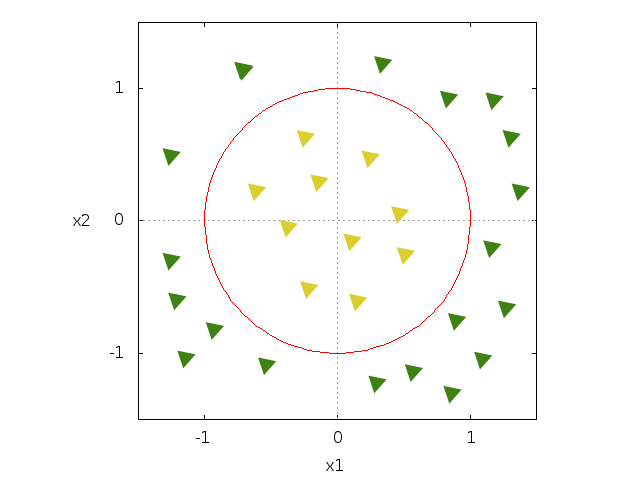
\includegraphics[scale=0.3]{./pictures/1.png} & 
\begin{eqnarray}
\notag h_\theta(x) &=& \theta_0 + \theta_1 x_1 + \theta_2 x_2 + \theta_3 x_3 +\theta_4 x_4 \\
\notag \theta &=& \begin{bmatrix}
-1 & 0 & 0 & 1 & 1
\end{bmatrix} 
\end{eqnarray}
\end{tabular}
%\caption{Example of decision boundary}
\end{table}

But what if our decision boundary was not fitting the data correctly. Then we have to change model parameters. For this purpose we must first define cost function for this model which we derive from statistics principle of maximum likelihood estimation.

\begin{equation}
\begin{aligned}
cost(h_\theta(x), t) &=& -tlog(h_\theta(x))-(1-t)log(1-h_\theta(x)) \\
cost(h_\theta(x), t) &=& \left\{
  \begin{array}{l l}
    -log(h_\theta(x)) & \quad \text{if \(t = 1\)}\\
    -log(1-h_\theta(x)) & \quad \text{if \(t = 0\)} 
  \end{array} \right.
\end{aligned}
\end{equation}

This cost function penalize hypothesis for wrong answers. If we plot this log functions we will see that cost for wrong answers is exponentially growing to infinite and cost for correct answers is 0 giving us a nice gradients which we later use to optimize this cost function. By knowing that we want to minimize cost function for our data set (\(m\) stands for one training case). In chapter below I will describe Gradient Descent algorithm for minimizing cost function.

\begin{equation}
J(\theta) = \frac{1}{m}\sum\limits_{i=1}^m cost(h_\theta(x)^i, t^i)
\end{equation}

Multiclass classification is done by one-vs-all method sometimes called one-vs-rest. Basically we will divide our classification problem into set of binary classification problems. We will then train multiple classifiers (number of classifiers is the same as the number of classes \(c\)) each one producing his own \(h_\theta^c(x)\). We will not apply the threshold thus our hypothesis is computing the probability of \(h_\theta^c(x) = c\). As a output we will pick most certain classifier.

\section{Gradient descent}
Gradient descent is model optimization algorithm which is trying to fit model parameters according to data by minimizing cost function. If cost function we are trying to minimize is convex we are guaranteed that function has only one minimum (global minimum). If not we can find sub optimal solution by ending up in local minimum. Backbone of this algorithm is very simple.

\begin{enumerate}
\item Initialize model parameters
\item Keep changing model parameters by minimizing cost function until we find a minimum
\end{enumerate}

\begin{algorithm}[h]
\Repeat{converge}{
\(TMP\theta_j = \theta_j - \alpha \frac{\partial}{\partial \theta_j}J(\theta_0, \theta_1, \dots)\)  \\
\(\theta_j = TMP\theta_j\)
}
\end{algorithm}

Where \(\alpha\) is learning rate which is telling us how big our step will be, derivative term is direction  of steepest descent. Algorithm is implemented with simultaneous update of parameters since updating one parameter affects rest of them. You should try different learning rates for your problem, usually we initialize \(\alpha\) with small number for example 0.001. If we set learning rate too big there is a possibility to overshoot minimum and algorithm may fail to converge or even diverge. With proper(small enough) learning rate fixed, algorithm is guaranteed to converge and not overshoot the minimum because derivatives get smaller as we are approaching to minimum. On the other hand choosing learning rate too small makes algorithm to converge very slowly.

Testing that algorithm is working correctly can be done by plotting cost function  as number of epoch (epoch is one run over training set) done. We should see that cost function is decreasing every iteration. Or we may come up with more automatic way when we sample from cost function and check if we converged. Usually we declare convergence when step is smaller than \(10^{-3}\) but this is state of preference.  We can speed up Gradient descent if we use some data normalization techniques such as Mean normalization and Feature scaling for more details see. 

Gradient Descent isn't only algorithm to minimize cost function parameters. Here is a list of some more complex algorithms where we usually don't care about learning rate alpha and they are usually faster. Also analytical solution exists, it's called normal equation. It is correct to use it when we don't have many features because it might become very computational intensive. For more details about normal equation see this.

\section{Regularization}
While we are trying to fit some decision boundary to our dataset we may find that our function is not generalizing well. That mean we have good results on our training set but results on test set are poor. This problem is called overfitting. One solution to this problem is to reduce magnitude of model weights. By this function smoothing our hypothesis will become simpler and possibly will generalize better. We do this by adding this \(\lambda\) term to our logistic cost function which is iterating over our model parameters.

\begin{equation}
-\frac{1}{m}[\sum\limits_{i=1}^m t^i log(h_\theta(x^i)) + (1-t^i) (1 - log(h_\theta(x^i)))] + \frac{\lambda}{2m}\sum\limits_{j=1}^n \theta_j^2 
\end{equation}

Character \(\lambda\) is our regularization term which is controlling trade-off between fitting our data well and keeping magnitude of weights small. See that we don't usually regularize the bias term \(\theta_0\). Have this in mind when implementing Gradient descent.

\chapter{Neural networks}
\section{Non-linear hypothesis}
Now we know about Logistic regression classification algorithm which with Gradient descent or some other optimization technique can calibrate very complex non-linear decision boundary by fitting many polynomial terms to cross any sort of data. So what is a flaw of this algorithm that resulted in need more sophisticated algorithms like neural network. It turns out that for many machine learning problems we need a huge amount of features to learn properly and we certainly don't want to handcraft them to make logistic regression work well. We want some algorithm to do this work for us.

For example if we only use all quadratic features overall number of features will growth \(O(n^2)\) and expression strength might be not so great. If we would use cubic features number of features will increase \(O(n^3)\). By knowing that we would like to recognize objects in small \(50 \times 50\)  grayscale images where every pixel is one input feature. Than only for quadratic features this number goes to nearly \(3\times 10^6\) and for cubic ones approximately \(2.6\times 10^9\). We can come up with only subset of those but we are not sure how this subset would look like. 

\section{Architecture}
Basic computational unit of neural network is neuron. These neurons are connected to network by synapses. Neuron can have multiple input called dendrites which are collecting input from other neurons creating dendritic tree. Output is called axon and is only one but can branch multiple times leading his signal to synapses. Neurons are then influenced by other neurons. To which degree is dependent on strength of synapses between them. This can dynamically change as we are observing new things. By this adaptation neural network is learning to perform useful computation. 

\begin{center}
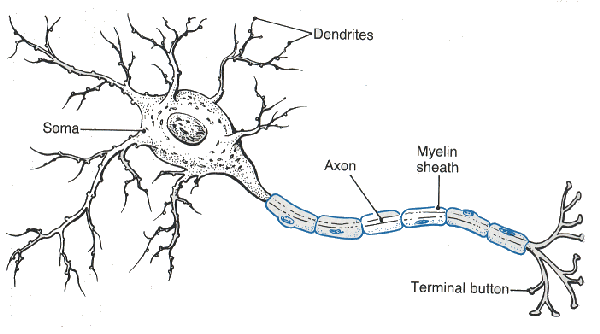
\includegraphics[scale=0.3]{./pictures/2.png}
\end{center}

Here is model of artificial neuron. The synaptic strength is modeled by weights, sometimes called parameters. These parameters are represented by numbers assigned to each input connection. Take note of a extra bias parameter which allows us to set a threshold for neuron activation function.

\begin{center}
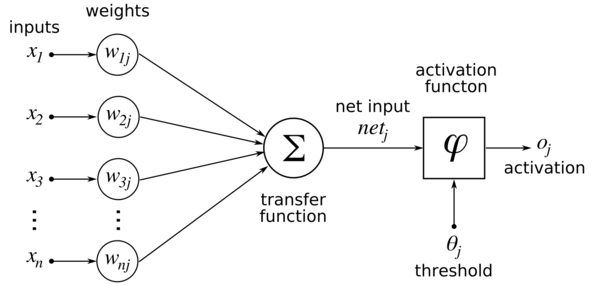
\includegraphics[scale=0.3]{./pictures/3.png}
\end{center}

Neuron takes his input multiplied by the weight and add the bias term. On result will apply some non-linear function. This is very simplified model of computation that biological neuron does. If our neuron would have logistic activation function that would be exactly the same as a logistic regression unit. We would not computed hypothesis but only activation for this neuron. 

\begin{eqnarray}
z = b + \sum\limits_{i=1}^j w_i x_i \quad
a = \frac{1}{1 + e^{-z}}
\end{eqnarray}

To compute complete hypothesis we need to create architecture from neurons. The most commonest one is feed-forward neural network. This is standard architecture for object recognition and one that we will use for my experiments. First layer is called input layer, the last one is called output layer. Layer in between are called hidden layers. If there are more then one hidden layers we call this deep neural network. Every Layer is computing activation function for its neurons by applying some non-linear function to activations coming from layer below.

Another architecture is recurrent neural network which are much more powerful than feed-forward nets. They are containing directed cycles between their connections making them suitable for modeling sequential data. Also they have ability to remember information for a long time and are more biologically realistic. There are many more architectures, usually deviation from this two above but I will focus only on describing feed forward networks suitable for object recognition.

\begin{figure}[h]
\centering
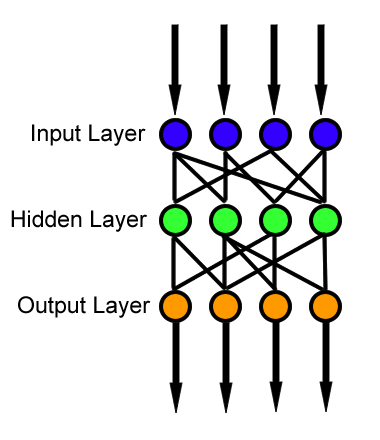
\includegraphics[scale=0.4]{./pictures/4.png}
\caption{Picture of feed-forward neural network}
\end{figure}

\section{Learning}
While learning neural network we are converting input into set of features and these features to final hypothesis. Think about this features as a neuron activations. We than have an ability to tune them by weighting(modeling synaptic strength). To do correct tuning we need an algorithm for multilayer neural networks which is measuring impact of changing each weight on our hypothesis. This algorithm is called backpropagation.

Learning of neural network can be done in different ways. There is supervised learning which we saw in our previous logistic regression training - providing training data where every sample is containing correction signal. It is common to use this in classification and regression tasks. In unsupervised learning we are feeding our model with raw data without correction hoping that our model will find good internal representation. One way to do this is by usage of autoencoders see. It is often used to enhance performance as pretraining when we initialize model parameters using unsupervised learning and then finetune it with supervised learning. Reinforcement learning is using reward system to influence model behavior.

\section{Cost function}
First we define our optimization objective. We will use multinomial logistic regression cost function sometimes called cross entropy cost function. U may see that this is just generalization of our logistic regression cost function for multiple output hypothesis.

\begin{equation}
-\frac{1}{m}[\sum\limits_{i=1}^m \sum\limits_{k=1}^K t^i_k log(h_\theta(x^i))_k + (1-t^i_k) (1 - log(h_\theta(x^i))_k)]
\end{equation}

Considering that we have more than just two classes we are now comparing two vectors whose size is equal to number of classes we are recognizing. First vector  belonging to our output layer is telling us what is our hypothesis for k-th output unit. Second is our correction signal for our output layer. If we add regularization term to our cost function it will look like this. We added iteration over every weight in all units and layers. This regularization term is often called weight-decay.

\begin{equation}
-\frac{1}{m}[\sum\limits_{i=1}^m \sum\limits_{k=1}^K t^i_k log(h_\theta(x^i))_k + (1-t^i_k) (1 - log(h_\theta(x^i))_k)] + \frac{\lambda}{2m}\sum\limits_{l=1}^L \sum\limits_{u=1}^U \sum\limits_{w=1}^{U+1}(\theta^l_{uw})^2 
\end{equation}

Often u may see different cost functions like squared error. It's proper to used them with linear units because you get much worse gradients when you are moving in nearly flat areas of logistic activation function.

\begin{equation}
\frac{1}{2m}\sum\limits_{i=1}^m(h_\theta(x^i) - t^i)^2
\end{equation}

\section{Softmax output layer}
This layer is used in classification tasks as a output layer and is combined with cross entropy cost function. Every neuron in this layer is representing one exclusive class and these neurons are representing probability distribution over all exclusive classes. Activation function is \(e^z\). Sum over all unit outputs \(y_i\) must be 1. This is done by bottom term.

\begin{equation}
y_i = \frac{e^z}{\sum\limits_{i=1}^m e^z_i}
\end{equation}

We are usually trying to avoid big softmax unit unless we have a huge dataset as it might contain lot of extra weights a than cause overfitting. For further information see this [Collober Weston 2008].

\section{Backpropagation}
Now we have our neural net architecture set for classification. It can contain many layers ended by output softmax layer which is representing probability distribution over all mutually exclusive classes. Our hidden layers are representing learned features. We now want to learn this model to provide us useful features for our problem. In order to do this we need to feed our gradient descent algorithm with partial derivatives which are telling us what is a direction of steepest descent for our model parameters. Efficient algorithm to compute derivatives in deep neural net is called backpropagation.

Idea behind this algorithm is that we can measure how much is error changing as we are tuning hidden activity. This activity can have various effects on other activities therefore many different effects on cost function. These effects must be combined. To do this we are using chain rule to gradually get derivatives for all weights to feed our gradient descent algorithm. This procedure is very similar to forward pass.

\begin{equation}
\frac{\partial J_m}{\partial y_m} = \frac{y_m - t_m}{y_m (1 - y_m)}
\end{equation}

First we compute how is our cost function changing as we are changing its input for training case \(m\). Then we are getting to our softmax layer and at first we have to compute how is our output \(y_i\) changing when we change activation of our unit \(i\).

\begin{equation}
\frac{\partial y_i}{\partial z_i} = y_i (1 - y_i)
\end{equation}

Now we will use chain rule in order to compute how is our cost function changing with respect of activation of unit \(i\) in softmax group.  Notice that we have to add up over all units in group because when we change logit \(z_i\) output of all other units changes.

\begin{equation}
\frac{\partial J}{\partial z_i} = \sum\limits_j\frac{\partial J}{\partial y_j}\frac{\partial y_j}{\partial z_i} = y_i - t_i
\end{equation}

So equation is saying how fast our cost function changes as we change output of a unit \(j\) times how fast is output of a unit \(j\) changes as we change logit \(z_i\). Finally we will apply this chain rule to every connection in our neural network. For logistic units derivatives will looks like this and when we have activation derivatives its simple to get derivatives with respect of weights and input.  

\begin{eqnarray}
\frac{\partial y}{\partial z} = y(1 - y) \\
\frac{\partial z}{\partial x_i} = w_i \quad \frac{\partial z}{\partial w_i} = x_i
\end{eqnarray}

\section{Model initialization}
Neural networks needs to initialize their parameters randomly in order to force neurons compute different features. This problem is referred as a symmetry breaking. Neurons initialized with the same bias and same incoming and outgoing weights gets the same gradients even after we ran gradient descent. We then have to initialize weights with some random values that are close to zero.

[Geoff Hinton] is suggesting that this values should be chosen as a proportion to square root of unit fan-in. Because if hidden unit would have big fan-in even small changes of incoming weights may have a big impact on its learning and perhaps we may overshoot.

\section{Scaling gradient descent with large dataset}
Now we have computed derivatives of our cost function using backpropagation algorithm and we can optimize our cost function using gradient descent. Particularly if we use large dataset we may find that this might be very computationally expensive. Problem is that in order to make a step toward steepest descent we require to compute average cost for whole training set. This default version is called batch gradient descent and may require to load lot of data from memory in order to gradually compute summary in. Instead we might use stochastic gradient descent which is updating parameters after every training sample. It is very important to  randomly shuffle dataset first to make our training generalize. Note that some weight changes take us farther from local optima but this version is way faster because we are making many steps in just one loop over training set. Particularly if we are working with highly redundant data. Alternatively we may use mini-batch gradient descent when we divide our training data into set of mini-batches and taking step after each iteration over them. This might be even faster than stochastic gradient descent if we use proper vectorized implementation.

Another way how to speed learning is to choose proper learning rate \(\alpha\). We might come up with several ideas in order to tune \(\alpha\). If we found that our error rate is fluctuating we might turn down learning rate. At the end of mini-batch learning it is always a good idea to do because variation in batches will cause fluctuation on weights. Or we might found that our error rate is continuously decreasing then we can increase learning rate.

Today commonest recipe for neural network learning is using mini-batch gradient descent combined  with momentum. Momentum is a method which is reducing gradient fluctuation and amplifies size of a steps in which gradients are stable. You can imagine its function as when you trying to change direction of a moving ball. It will deflect but its velocity makes it that it will partly continue in its previous direction. First we will compute momentum on training sample \(t\) and than we will update the weights by this value. Current gradient will increase previous velocity which is also decaying by \(\omega\) parameter set slightly lower than 1.

\begin{equation}
\begin{aligned}
v(t) &= \omega v(t-1)-\alpha\frac{\partial J}{\partial w} \\
\delta w(t) &= v(t)
\end{aligned}
\end{equation}

At the start of a training its good to set momentum to small value(e.g. 0.5) because gradients in this phase may highly fluctuate. When our learning has settled up we may rise momentum to its final value (0.9, 0.99). Also one nice property of momentum is that we can successfully learn with higher learning rate. For some more depth about momentum method I recommend to check Ilya Sutskever research [Ilya research]. 

\section{Dropout}
Dropout is a new technique which reduces overfitting by taking geometric mean from predictions of many models without separately training them. Presenting training case to our neural net we randomly omit each neuron in hidden layers with probability 0.5. By doing this we are forcing neuron to adapt his activation with different neurons every time we present training case. This makes him to more likely learn something useful and not so much reliant on opinion of his siblings. Combination of models is a good way to reduce test error particularly if our model predictions differ a lot. Considering dropout ration 0.5 on hidden unit we are sampling predictions from one of the \(2^U\) (\(U\) stands for the number of hidden units) models every training sample. We use shared weight for all these models to train them. At test time we are halving all outgoing weights to efficiently compute approximation of geometric mean.

We can do the same trick for input layer usually with lower probability ratios in fact this trick is already used in denoising autoencoders for preventing autoencoder to learn identity rather then features. Hinton is suggesting that is better to use model that have high variance(is likely to overfit) and combine it with dropout than smaller model with smaller capacity. That assuming we have enough computation power. For more information about droupout see[Hinton].

\chapter{Convolutional neural networks}
In literature are these networks often called Multi-stage Hubel Wiesel models referring that this architecture mimics functionality of simple and complex cells. Having multiple stages of feature detectors seems very natural approach for computer vision when we are usually thinking about object as a set of a simpler objects. At bottom of this architecture we might recognize edges, which are similar to Gabor filters, then motifs and towards the end objects. Each stage of this Multi-stage Hubel Wiesel architecture contains filter bank layer, non-linearity layer and pooling layer. At first stages of this architecture are learned filters usually similar to Gabor's filters.

\begin{figure}[h]
\centering
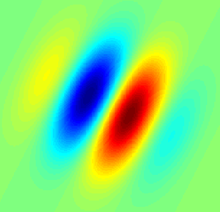
\includegraphics[scale=0.2]{./pictures/6.png}
\caption{Picture of 2D Gabor filter}
\end{figure}

\section{Architecture}
Filter bank layer is containing set of  maps where every map is containing copies of one feature detector. Each map is covering whole input space and its output is representing extracted features at all locations of input. Feature detector is a neuron with shared weights with his siblings in map. A nice property of this weight sharing is that we are massively reducing number of free parameters to work with in our network. It's usually very expensive to use filter with miscellaneous scales and rotations in map. Much easier solution is to work with your input data.

Non-linearity layer is encoding features by applying some kind of non-linear function. Common function is a pointwise tanh but recent experiment's showed that rectified sigmoid might be superior at least in natural image recognition[see]. Often is in combination with rectified sigmoid, or any other unbounded function, used response normalization which enforces competition between features in the same location.

Pooling layer is working with each map separately taking region of feature detectors activities and encoding them to more complex features. During this process we are reducing resolution on our input so we can afford to have more feature maps in layers above. Pooling process is providing us spatial invariance but has a disadvantage that we are loosing information about precise position of our features. This can be overcome to some extend by making this pooling regions overlap.

\begin{figure}[h]
\centering
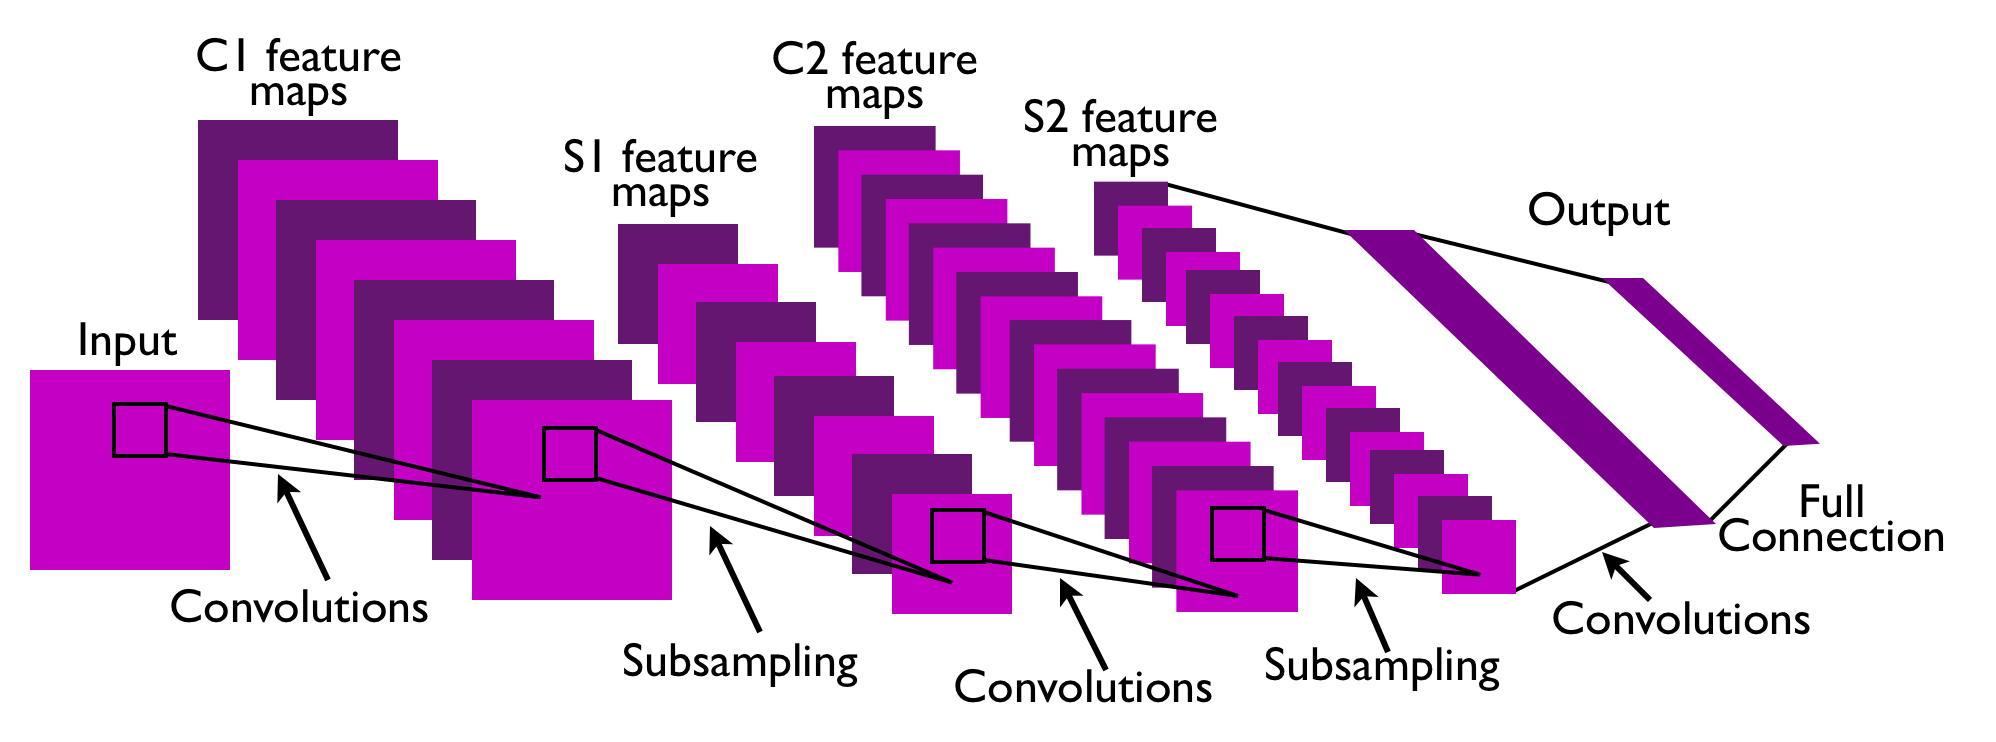
\includegraphics[scale=0.15]{./pictures/5.png}
\caption{Picture of convolutional neural network}
\end{figure}

On top of this staged architecture its common to have several fully connected layers before our softmax layer which are representing vectors of learned features.

\section{Learning}
Supervised learning is usually done by using mini-batch gradient descent with momentum. Gradients are computed with slightly modified backpropagation algorithm. Dropout is on these  types of net less effective due to weight sharing but still will be huge factor on large nets[ILSVRC-2012]. Unsupervised learning is used as a pretraining for enhancing our performance and good initialization for supervised fine tuning.

Modification of backpropagation algorithm has to count with weight sharing. We will initialize weights on same values and compute the gradients as usual. Then we will modify gradients by applying linear constraint. Our weights then will be equal.

\begin{equation}
\begin{aligned}
Rule \Rightarrow w_1 &= w_2 \land \delta w_1 = \delta w_2 \\
\frac{\partial J}{\partial w_{tied}} &= \frac{\partial J}{\partial w_1} + \frac{\partial J}{\partial w_2}
\end{aligned}
\end{equation}

\section{What is missing in convolutional neural networks}
Convolutional neural networks are learning feature representation of objects but during pooling process they are loosing precise spatial information of active features. So they can learn what are parts of human body and then recognize these bodies but they can hardly assign identities to those bodies. Making pool overlapping helps a bit because we have a features duplicated in several pools. This makes us able to inaccurately tell where it is. Another flaw is that they are not able to understand changes in view point position. This leads us to need huge dataset where we are duplicating samples under different scales and orientations.

People are very good at both problems. American psychologist Irvin Rock has bring the evidence that our visual system is using coordinate frames to represent shapes[see]. So if we would have presented object we can immediately recognize his rotation if we have right coordinate frame. As well we know about precise spatial relations between objects parts. We would like to have neural network model this knowledge. One suggested solution is by using pose vectors[hinton].

\chapter{Experiments}
My experiments will focus on testing variety of techniques which can enhance performance of convolutional neural networks like different architectures, units, preprocessing techniques, hyperparameters. At first I took known architectures which performed well on used dataset. Then I tried to change hyperparameters and test their impact on performance.

\section{Caltech101}
To challenge biological systems and prove for our existing ones usage in real world tasks we are using datasets which are emulating natural environment by containing pictures with variety of objects, backgrounds, positioning, posing and lightning. While humans are easily dealing with this kind of variations it is still challenge for artificial systems. Another problem which is connected to deep learning and generalization is that we don't see what we have learned. So informations which is using our neural network to decide category of object is hidden and might be misleading.

Caltech101 is containing 9144 natural images of size approximately \(300\times200\). Picture are categorized to 102 categories(adding one additional background category) each one is containing about fifty images. The biggest categories are planes, motorbikes and faces. This dataset is available at \url{http://www.vision.caltech.edu/Image_Datasets/Caltech101/}. Here are mentioned some issues with Caltech. 

Standard approaches on this dataset are using fixed number of images in each category for training and testing. Popular number of training images: 1, 3, 5, 10, 15, 20, 30. Popular numbers of testing images: 20, 30. It is also suggested that you should track misclassified samples. The best systems on this dataset are above 60\% classification accuracy. 

\begin{figure}[h]
\centering
{\renewcommand{\arraystretch}{0}
\setlength{\tabcolsep}{0cm}
\begin{tabular}{c c c}
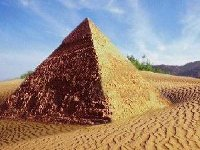
\includegraphics[scale=0.2]{./pictures/caltech_1.jpg} & 
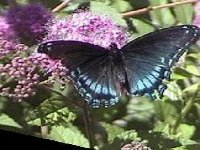
\includegraphics[scale=0.2]{./pictures/caltech_2.jpg} &

\includegraphics[scale=0.2]{./pictures/caltech_3.jpg} \\
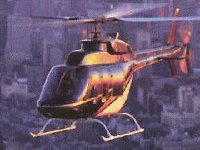
\includegraphics[scale=0.2]{./pictures/caltech_4.jpg} &
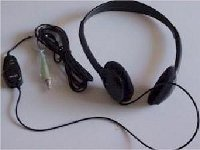
\includegraphics[scale=0.2]{./pictures/caltech_5.jpg} &
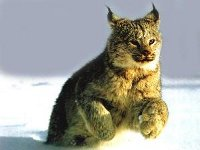
\includegraphics[scale=0.2]{./pictures/caltech_6.jpg}
\end{tabular}
}
\caption{Example of pictures from Caltech101}
\end{figure}